%~ \documentclass[letterpaper,times,draft]{sae}
\documentclass[letterpaper,times]{sae}

\usepackage[svgnames]{xcolor}
\definecolor{SAEblue}{RGB}{1,160,233}
%\raggedright

\usepackage[justification=justified, singlelinecheck=false]{caption}  % ,figurename=Fig.,labelfont={it}
\DeclareCaptionFont{eightpt}{\fontsize{8pt}{11pt}\selectfont #1}
\captionsetup{font={eightpt,color=SAEblue},labelsep=period}

\usepackage{lineno}
\usepackage[utf8]{inputenc}

\usepackage{array}% http://ctan.org/pkg/array (also necessary for width calculations (for vert. lines)))
\newcolumntype{L}[1]{>{\raggedright\let\newline\\\arraybackslash\hspace{0pt}}p{#1}}
\newcolumntype{C}[1]{>{\centering\let\newline\\\arraybackslash\hspace{0pt}}p{#1}}
\newcolumntype{R}[1]{>{\raggedleft\let\newline\\\arraybackslash\hspace{0pt}}p{#1}}

\usepackage{graphicx}
\graphicspath{{FIGURES/}}
\usepackage{cite}
\usepackage{multirow}
\usepackage{amsmath}

% Charge le module graphique tikz
\usepackage{tikz}
\usepackage{pgfplots}
\usetikzlibrary{backgrounds}
\usetikzlibrary{shapes,decorations,shadows,arrows,calc}
\usetikzlibrary{decorations.markings}

\newcommand{\ignore}[1]{}
\newcommand{\todo}[1]{\textcolor{red}{TODO: {#1}}}
\newcommand{\todr}[1]{\textcolor{purple}{CAN CUT: {#1}}}
\newcommand{\todm}[1]{\textcolor{green}{MOVE: {#1}}}
\newcommand{\case}[1]{\mbox{\textit{#1}}}
\newcommand{\textss}[1]{\textsuperscript{#1}}
\renewcommand{\deg}{$^\circ$}


\newcommand{\Figref}[1]{Figure \ref{#1}}
\newcommand{\Figrefs}[2]{Figures \ref{#1} and \ref{#2}}
\newcommand{\Figrefsto}[2]{Figures \ref{#1} to \ref{#2}}
\newcommand{\Tabref}[1]{Table \ref{#1}}
\newcommand*{\dt}[1]{%
\accentset{\mbox{\large\bfseries .}}{#1}}
\usepackage{nameref}
\usepackage{booktabs}

% Define "struts" as suggested by Claudio Beccari in
% a piece in TeX and TUG News, Vol. 2, 1993.
\newcommand\Tstrut{\rule{0pt}{4.6ex}}       % "top" strut
\newcommand\Bstrut{\rule[-0.9ex]{0pt}{0pt}} % "bottom" strut
\newcommand{\TBstrut}{\Tstrut\Bstrut} % top&bottom struts

%%% the following hides the section number while keeping their numbering for proper referencing in toc and \ref
\makeatletter
\def\@seccntformat#1{%
  \expandafter\csname c@#1\endcsname\c@section
  }
\makeatother

\usepackage{subfigure}
\usepackage{multimedia}

\DeclareMathOperator{\sign}{sign}
\newcommand{\quotes}[1]{``#1''}


\PaperTitle{A Level-Set Framework for Multilayer Aircraft Ice Accretion}
\usepackage{calc} % to get proper table widths (subtracting colsep and black lines width

\makeatletter 
\renewcommand\@biblabel[1]{#1. } 
\makeatother

%\AddAuthor{Karim Zayni}{Department of Mechanical Engineering, Polytechnique Montr\'{e}al, Montr\'{e}al, Canada}
%\AddAuthor{Eric Laurendeau}{Department of Mechanical Engineering, Polytechnique Montr\'{e}al, Montr\'{e}al, Canada}
\PaperNumber{2027-XX-XXXX}
%\SAECopyright{2027}



\begin{document}
\maketitle
% ============================================================
% ABSTRACT
% ============================================================

\begin{abstract}

This work presents a continuous level-set methodology for the prediction of multilayer aircraft ice accretion on unstructured meshes. Conventional multilayer icing simulations commonly update the ice geometry through explicit displacement of surface nodes, which can become sensitive to mesh quality as strongly curved and interacting ice features develop. The proposed methodology instead represents the evolving ice–air interface implicitly as the zero contour of a signed-distance level-set function. A key contribution of this work is the extension of the continuous level-set formulation to the prediction of complex 3D multilayer ice-accretion geometries. Implemented within the \textsc{CHAMPS} icing framework, the methodology combines surface-quantity propagation, semi-implicit Rosenbrock–Wanner (ROW) time integration, and conformal surface extraction using \textsc{MMG}. The methodology is assessed for representative 2D and 3D configurations from the AIAA Ice Prediction Workshops (IPW). The results demonstrate robust multilayer ice accretion in both 2D and 3D, with increasing numbers of accretion layers showing convergence of the predicted ice geometries toward experimental measurements.

\end{abstract}


% ============================================================
% INTRODUCTION
% ============================================================

\section{Introduction}

Aircraft ice accretion can significantly degrade aerodynamic performance by modifying the geometry of lifting surfaces \cite{CAO2018353}. Numerical icing simulations generally employ a quasi-steady multilayer approach in which aerodynamic, droplet-impingement, and thermodynamic solutions are successively recomputed as the ice geometry evolves \cite{KIND1998257}.

Geometry evolution remains an important numerical challenge. Conventional methods typically displace surface nodes along the local surface-normal direction \cite{thompsonDeformation}. Although computationally efficient, repeated normal displacement can lead to mesh distortion or entanglement as strongly curved or interacting ice features develop, particularly in 3D \cite{glimm2000,Ozcer_2019}.

Level-set methods represent evolving interfaces implicitly through a scalar field and provide a framework for tracking complex moving boundaries \cite{OSHER198812,OSHER2004,GIBOU201882}. They have been applied to moving-interface problems and, more recently, to aircraft ice accretion \cite{PENA2016278,sbcLevelSet,lavoieLevelSet,alessandroLevelSet}.

The present work develops a continuous level-set framework for 2D and 3D multilayer ice accretion within the \textsc{CHAMPS} solver \cite{champsArticle}. The significant aspect of the proposed approach is the evolution of the ice interface independently of the connectivity and displacement of the surface mesh, followed by conformal extraction and remeshing between successive accretion layers. This formulation is intended to improve robustness for complex 3D ice geometries and interacting ice fronts.


% ============================================================
% METHODOLOGY
% ============================================================

\section{Methodology}

The methodology is embedded within the quasi-steady icing framework shown in Fig.~\ref{fig:icingFramework}. For each layer, the aerodynamic flow, droplet impingement, and surface thermodynamics are computed sequentially. The resulting ice thickness drives the level-set evolution, after which the new surface is extracted and remeshed for the subsequent layer.

\begin{figure}[htb]
    \centering
    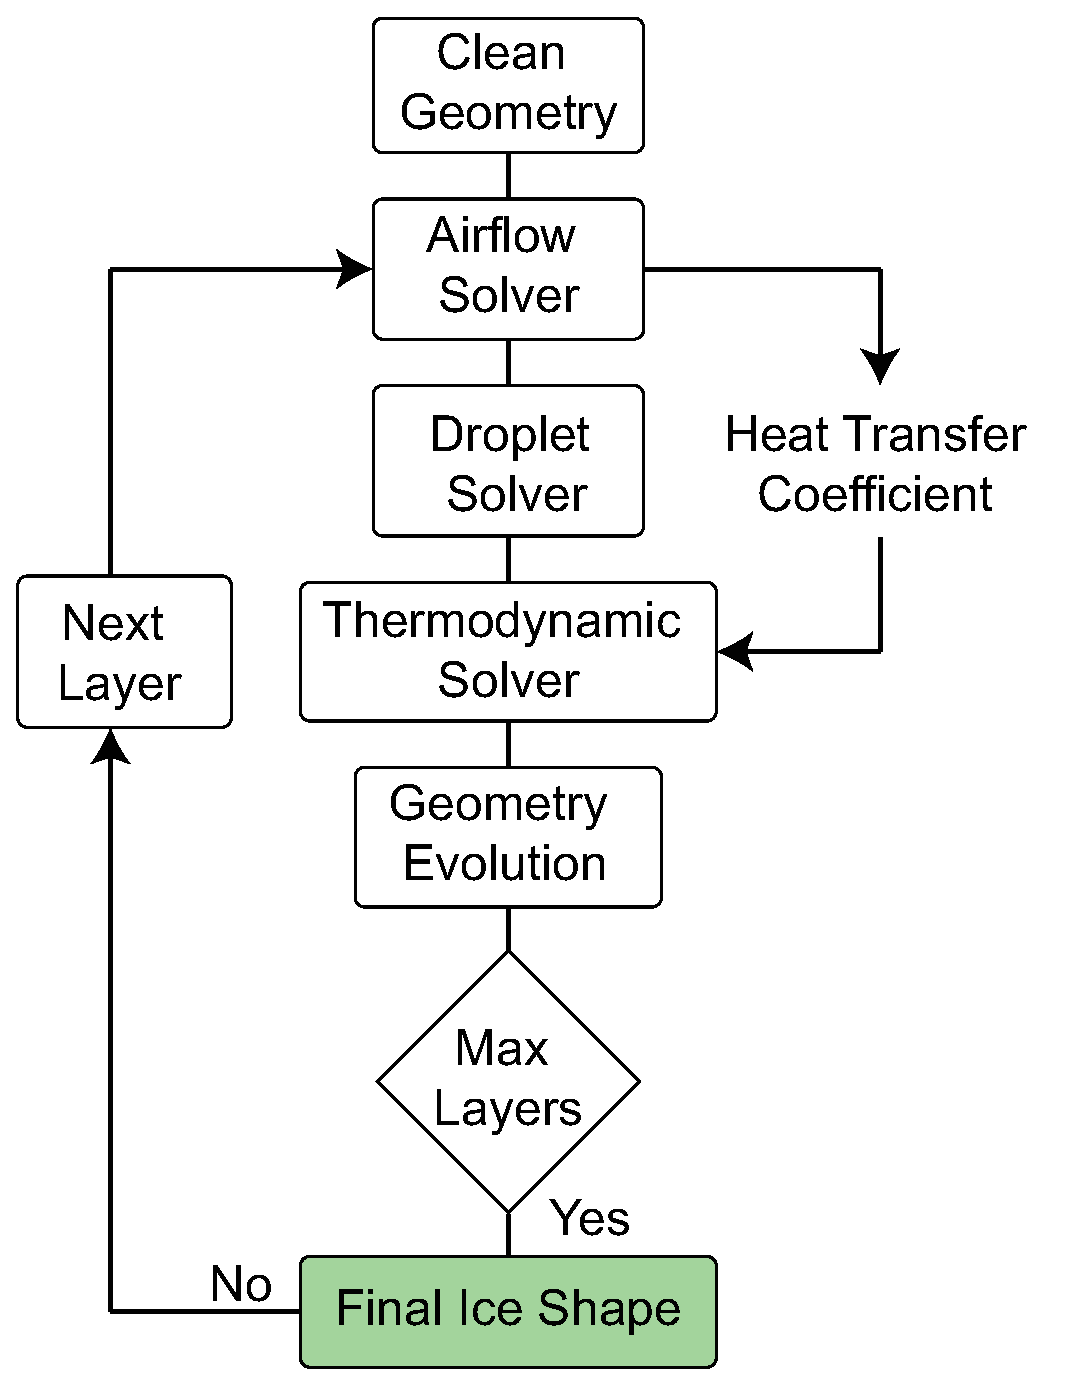
\includegraphics[width=0.6\linewidth]{icingFramework.eps}
    \caption{Quasi-steady multilayer ice-accretion framework implemented within \textsc{CHAMPS}.}
    \label{fig:icingFramework}
\end{figure}


% ------------------------------------------------------------
% Level-set representation
% ------------------------------------------------------------

\subsection{Interface Representation and Advection}

The ice--air interface is represented by a level-set function $\phi$, with $\phi<0$ in the ice, $\phi>0$ in the fluid, and $\phi=0$ at the interface, as illustrated in Fig.~\ref{fig:iceAirInterface}.

\begin{figure}[htb]
    \centering
    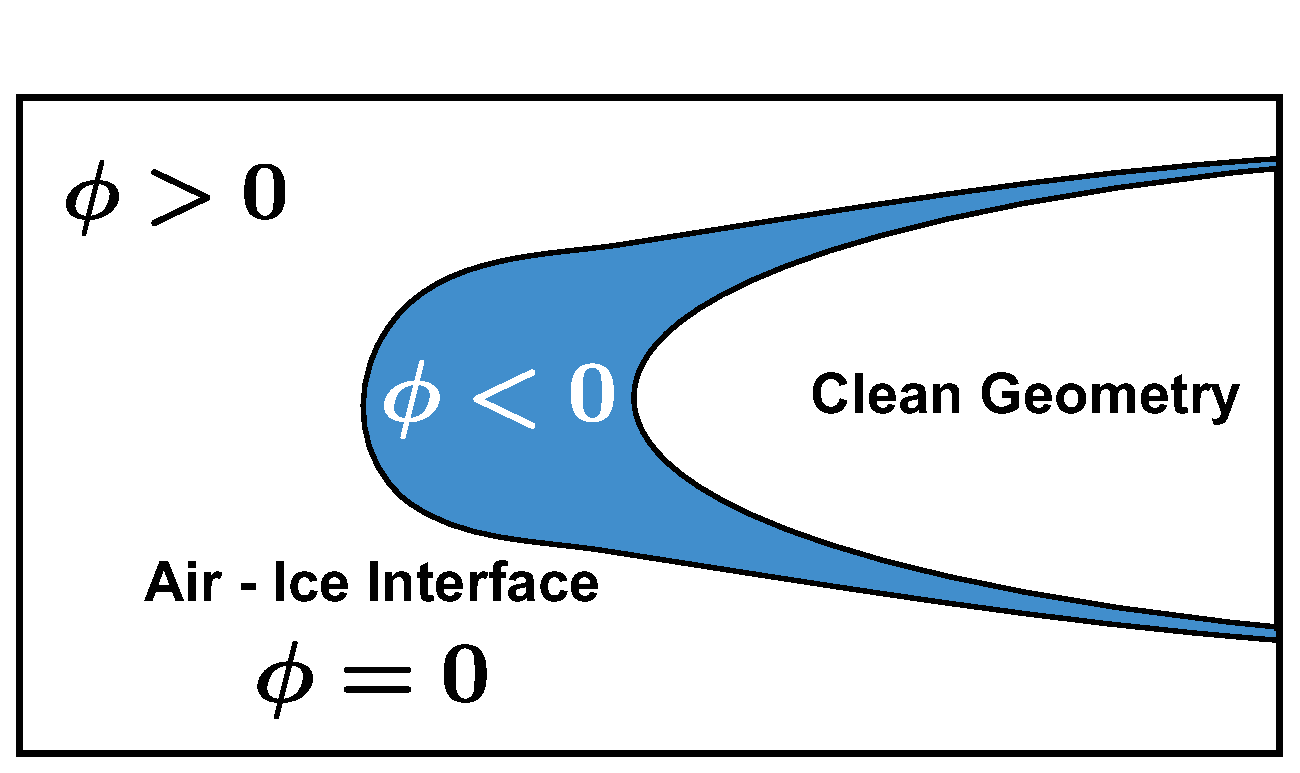
\includegraphics[width=0.60\linewidth]{FIGURES/ICE_AIR_INTERFACE.eps}
    \caption{Level-set representation of the ice--air interface.}
    \label{fig:iceAirInterface}
\end{figure}

The initial signed-distance field, illustrated in Fig.~\ref{fig:levelset}(a), is obtained from the Eikonal equation \cite{XIA2010},

\begin{equation}
    |\nabla\phi|=1,
    \qquad
    \boldsymbol{n}_{\phi}=\frac{\nabla\phi}{|\nabla\phi|},
\end{equation}

where $\boldsymbol{n}_{\phi}$ denotes the unit normal vector to the level-set contours. The interface is advected using the level-set equation \cite{OSHER2004},

\begin{equation}
    \frac{\partial\phi}{\partial t}
    +\boldsymbol{V}_{ice}\cdot\nabla\phi=0,
\end{equation}

where the ice-growth velocity is

\begin{equation}
    \boldsymbol{V}_{ice}
    =
    \frac{h_{ice}}{\Delta t_{\mathrm{layer}}}
    \boldsymbol{n}_{\phi}.
\end{equation}

Here, $h_{ice}$ is the local ice thickness and $\Delta t_{\mathrm{layer}}$ is the accretion-layer duration. As illustrated in Fig.~\ref{fig:levelset}(b), the surface ice thickness is propagated into the level-set domain along $\boldsymbol{n}_{\phi}$ prior to level-set advection.

\begin{figure}[htb]
    \centering

    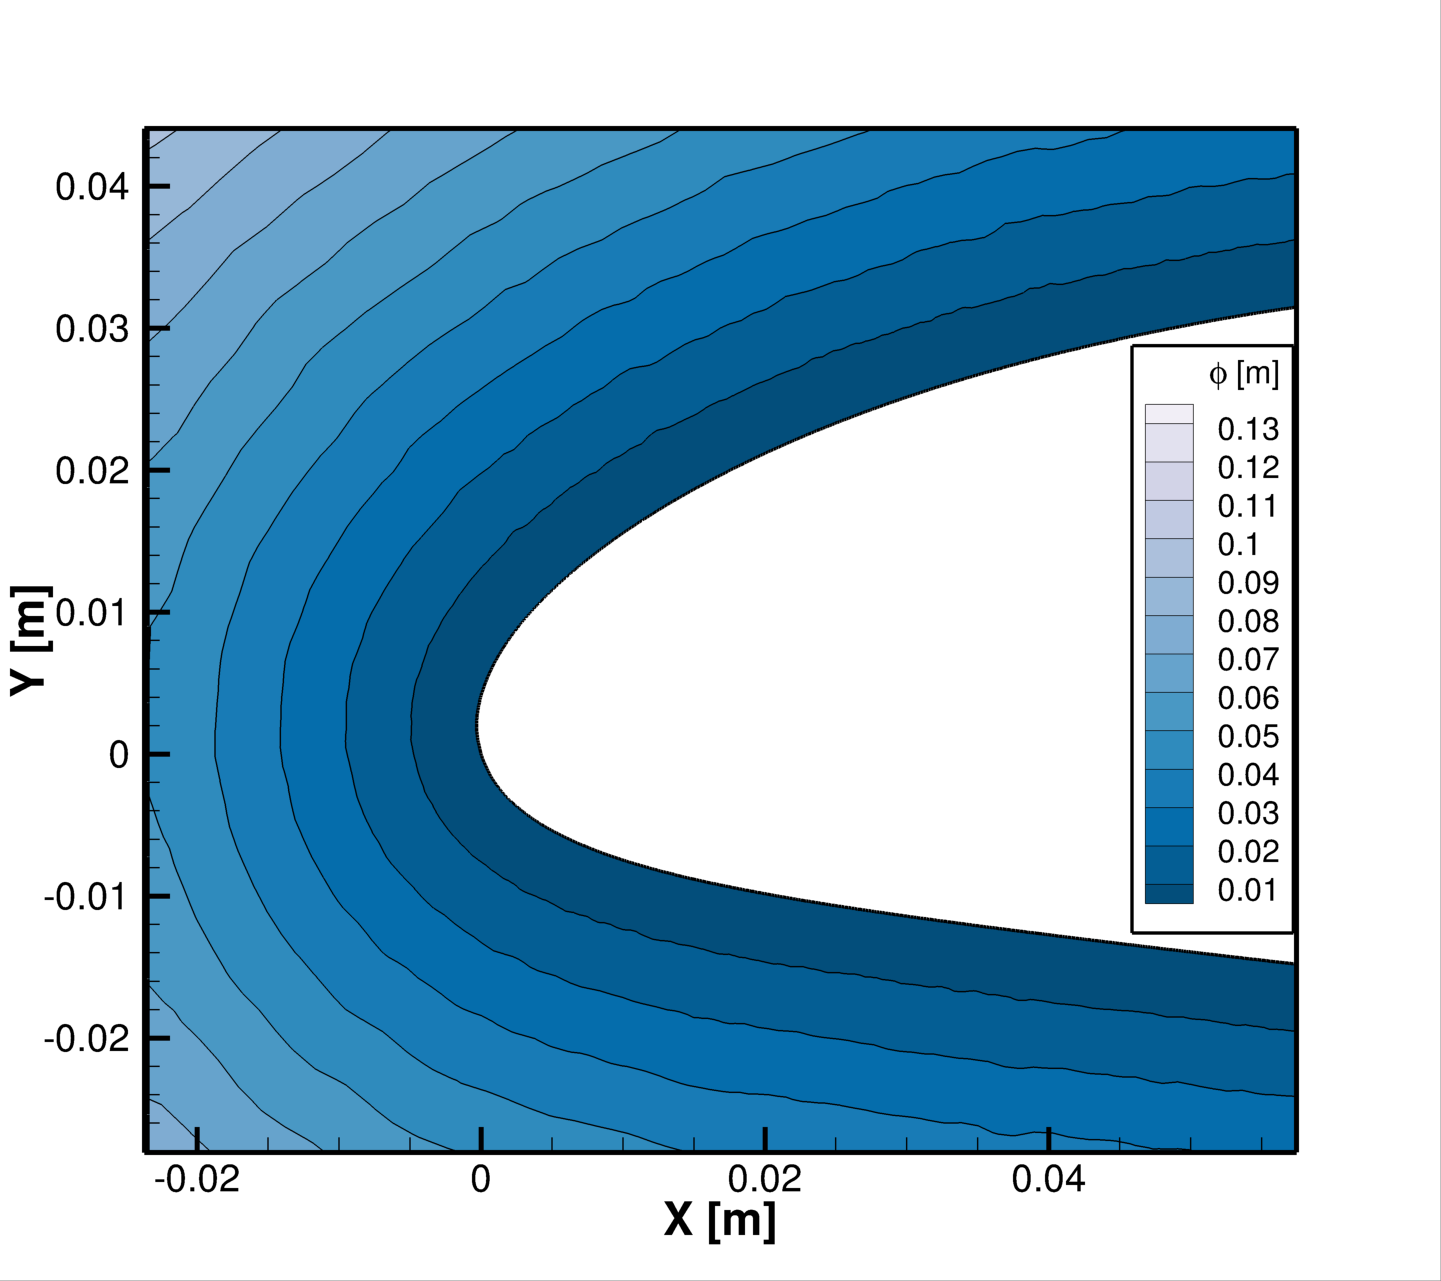
\includegraphics[width=0.75\linewidth]{EIKONAL.png}

    \small (a) Signed-distance initialization

    \vspace{0.15cm}

    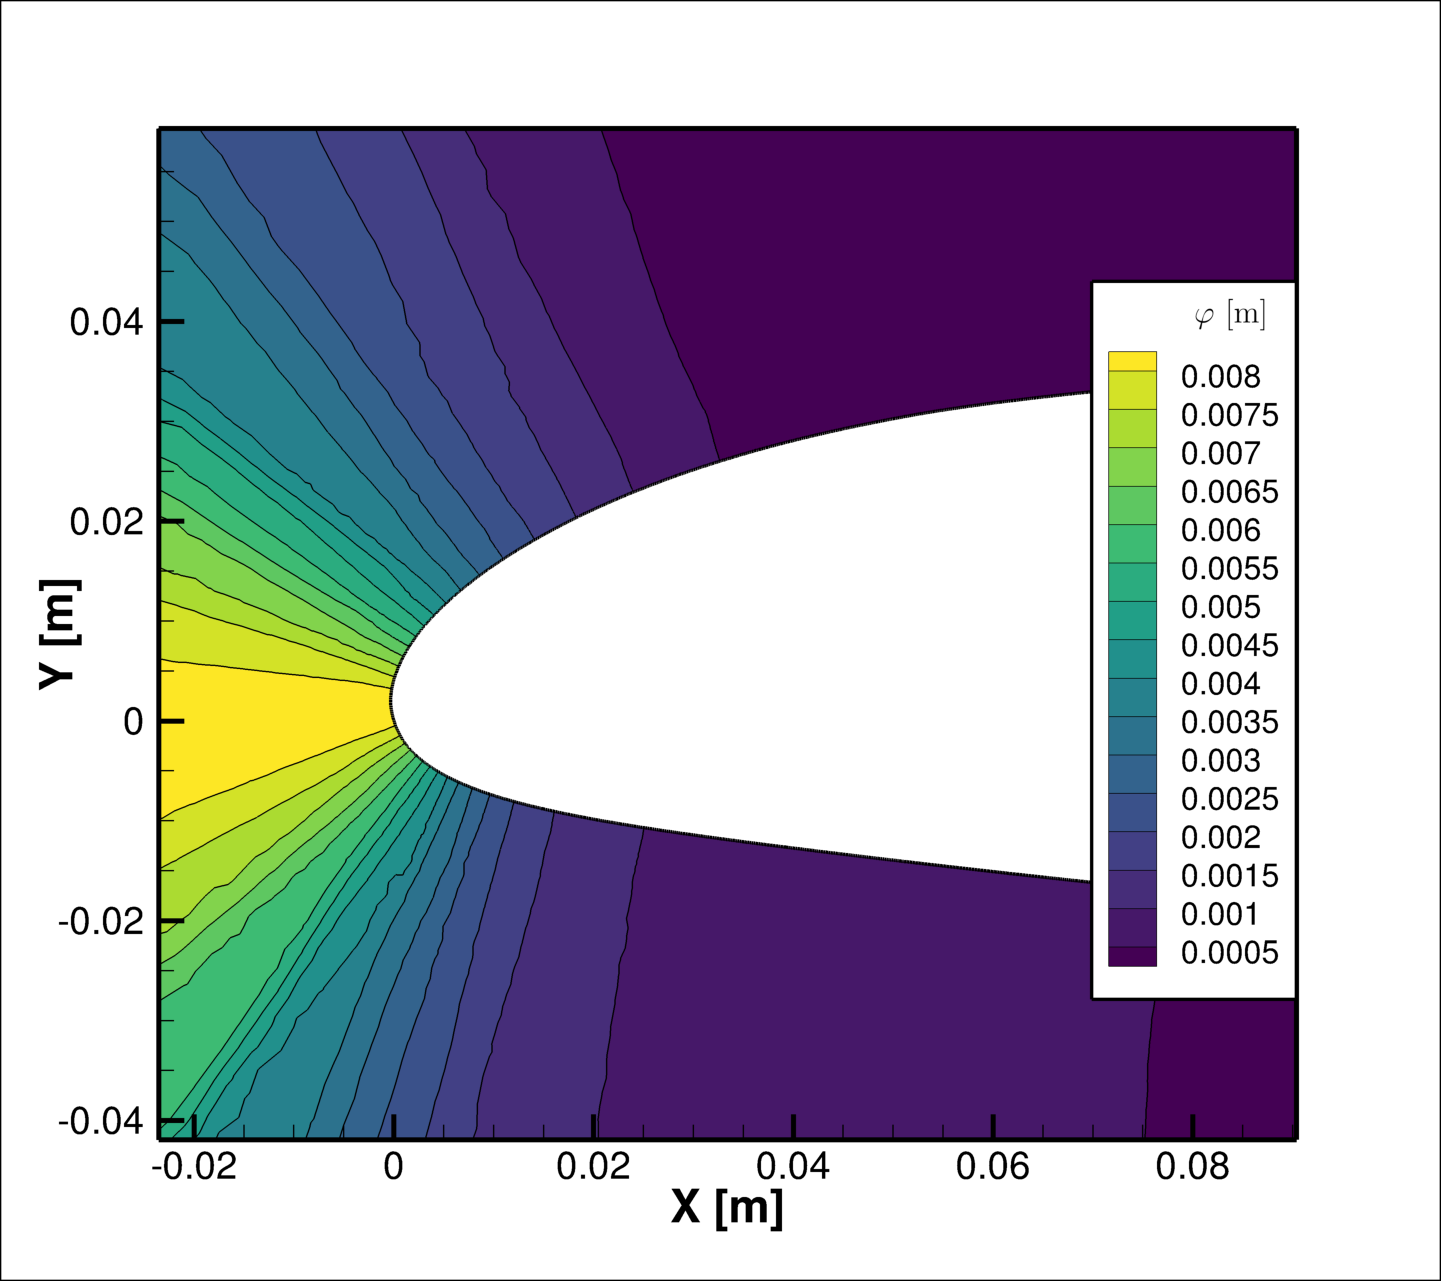
\includegraphics[width=0.75\linewidth]{PROPAGATION.png}

    \small (b) Ice-thickness propagation

    \caption{Level-set initialization and ice-thickness propagation prior to interface advection.}
    \label{fig:levelset}
\end{figure}


% ------------------------------------------------------------
% Time integration and surface extraction
% ------------------------------------------------------------

\subsection{Time Integration and Surface Extraction}

To alleviate restrictive time-step limitations associated with explicit level-set integration, the level-set equation is advanced using a two-stage semi-implicit Rosenbrock–Wanner (ROW) scheme \cite{hairer1996}. The time integration is written as

\begin{equation}
    \phi^{n+1}
    =
    \phi^n + \sum_{j=1}^{s} m_j S_j,
\end{equation}

where the stage increments $S_i$ are obtained from

\begin{equation}
    \left(
    \frac{\boldsymbol{I}}{\gamma\Delta t}
    +\boldsymbol{J}
    \right)^n S_i
    =
    -R\left(
    \phi^n+\sum_{j=1}^{i-1}a_{ij}S_j
    \right).
\end{equation}

Here, $R(\phi)$ is the spatial residual, $\boldsymbol{J}=\partial R/\partial\phi$ its Jacobian, and $S_i$ the stage increments. The resulting linear systems are solved using the Generalized Minimal Residual (GMRES) method \cite{saad1986gmres}. The semi-implicit formulation improves stability and permits larger time steps on the locally refined auxiliary mesh used for level-set advection, illustrated in Fig.~\ref{fig:meshAdaptation}. Following level-set advection, the $\phi=0$ interface is extracted using \textsc{MMG} \cite{DAPOGNY2014358} and remeshed for the subsequent accretion layer.

\begin{figure}[htb]
    \centering
    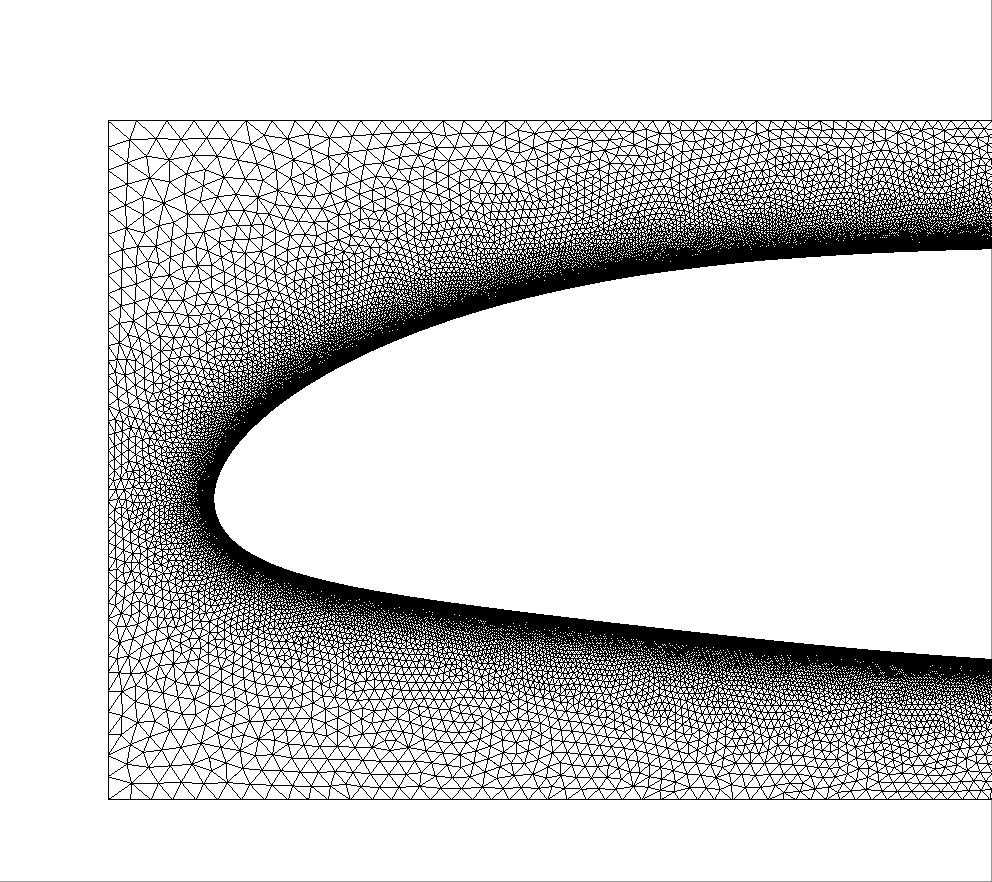
\includegraphics[width=0.72\linewidth]{FIGURES/MESH_ADAPTATION.png}
    \caption{Adapted auxiliary mesh with local refinement in the ice-accretion region for level-set advection.}
    \label{fig:meshAdaptation}
\end{figure}

% ============================================================
% PRELIMINARY RESULTS
% ============================================================

\section{Preliminary}

The methodology is first illustrated using the manufactured three-horn configuration introduced in \cite{pierreThermo}. This configuration features three distinct ice horns, producing highly concave and convex regions that challenge interface-tracking methods. An ice thickness of $0.02$~m is uniformly imposed on all surface nodes with $x<0.05$m. As shown in Fig.\ref{fig:threehorns}, direct surface displacement can lead to mesh entanglement as neighboring fronts interact, whereas the implicit level-set representation naturally accommodates their evolution and merging.

\begin{figure}[htb]
\centering
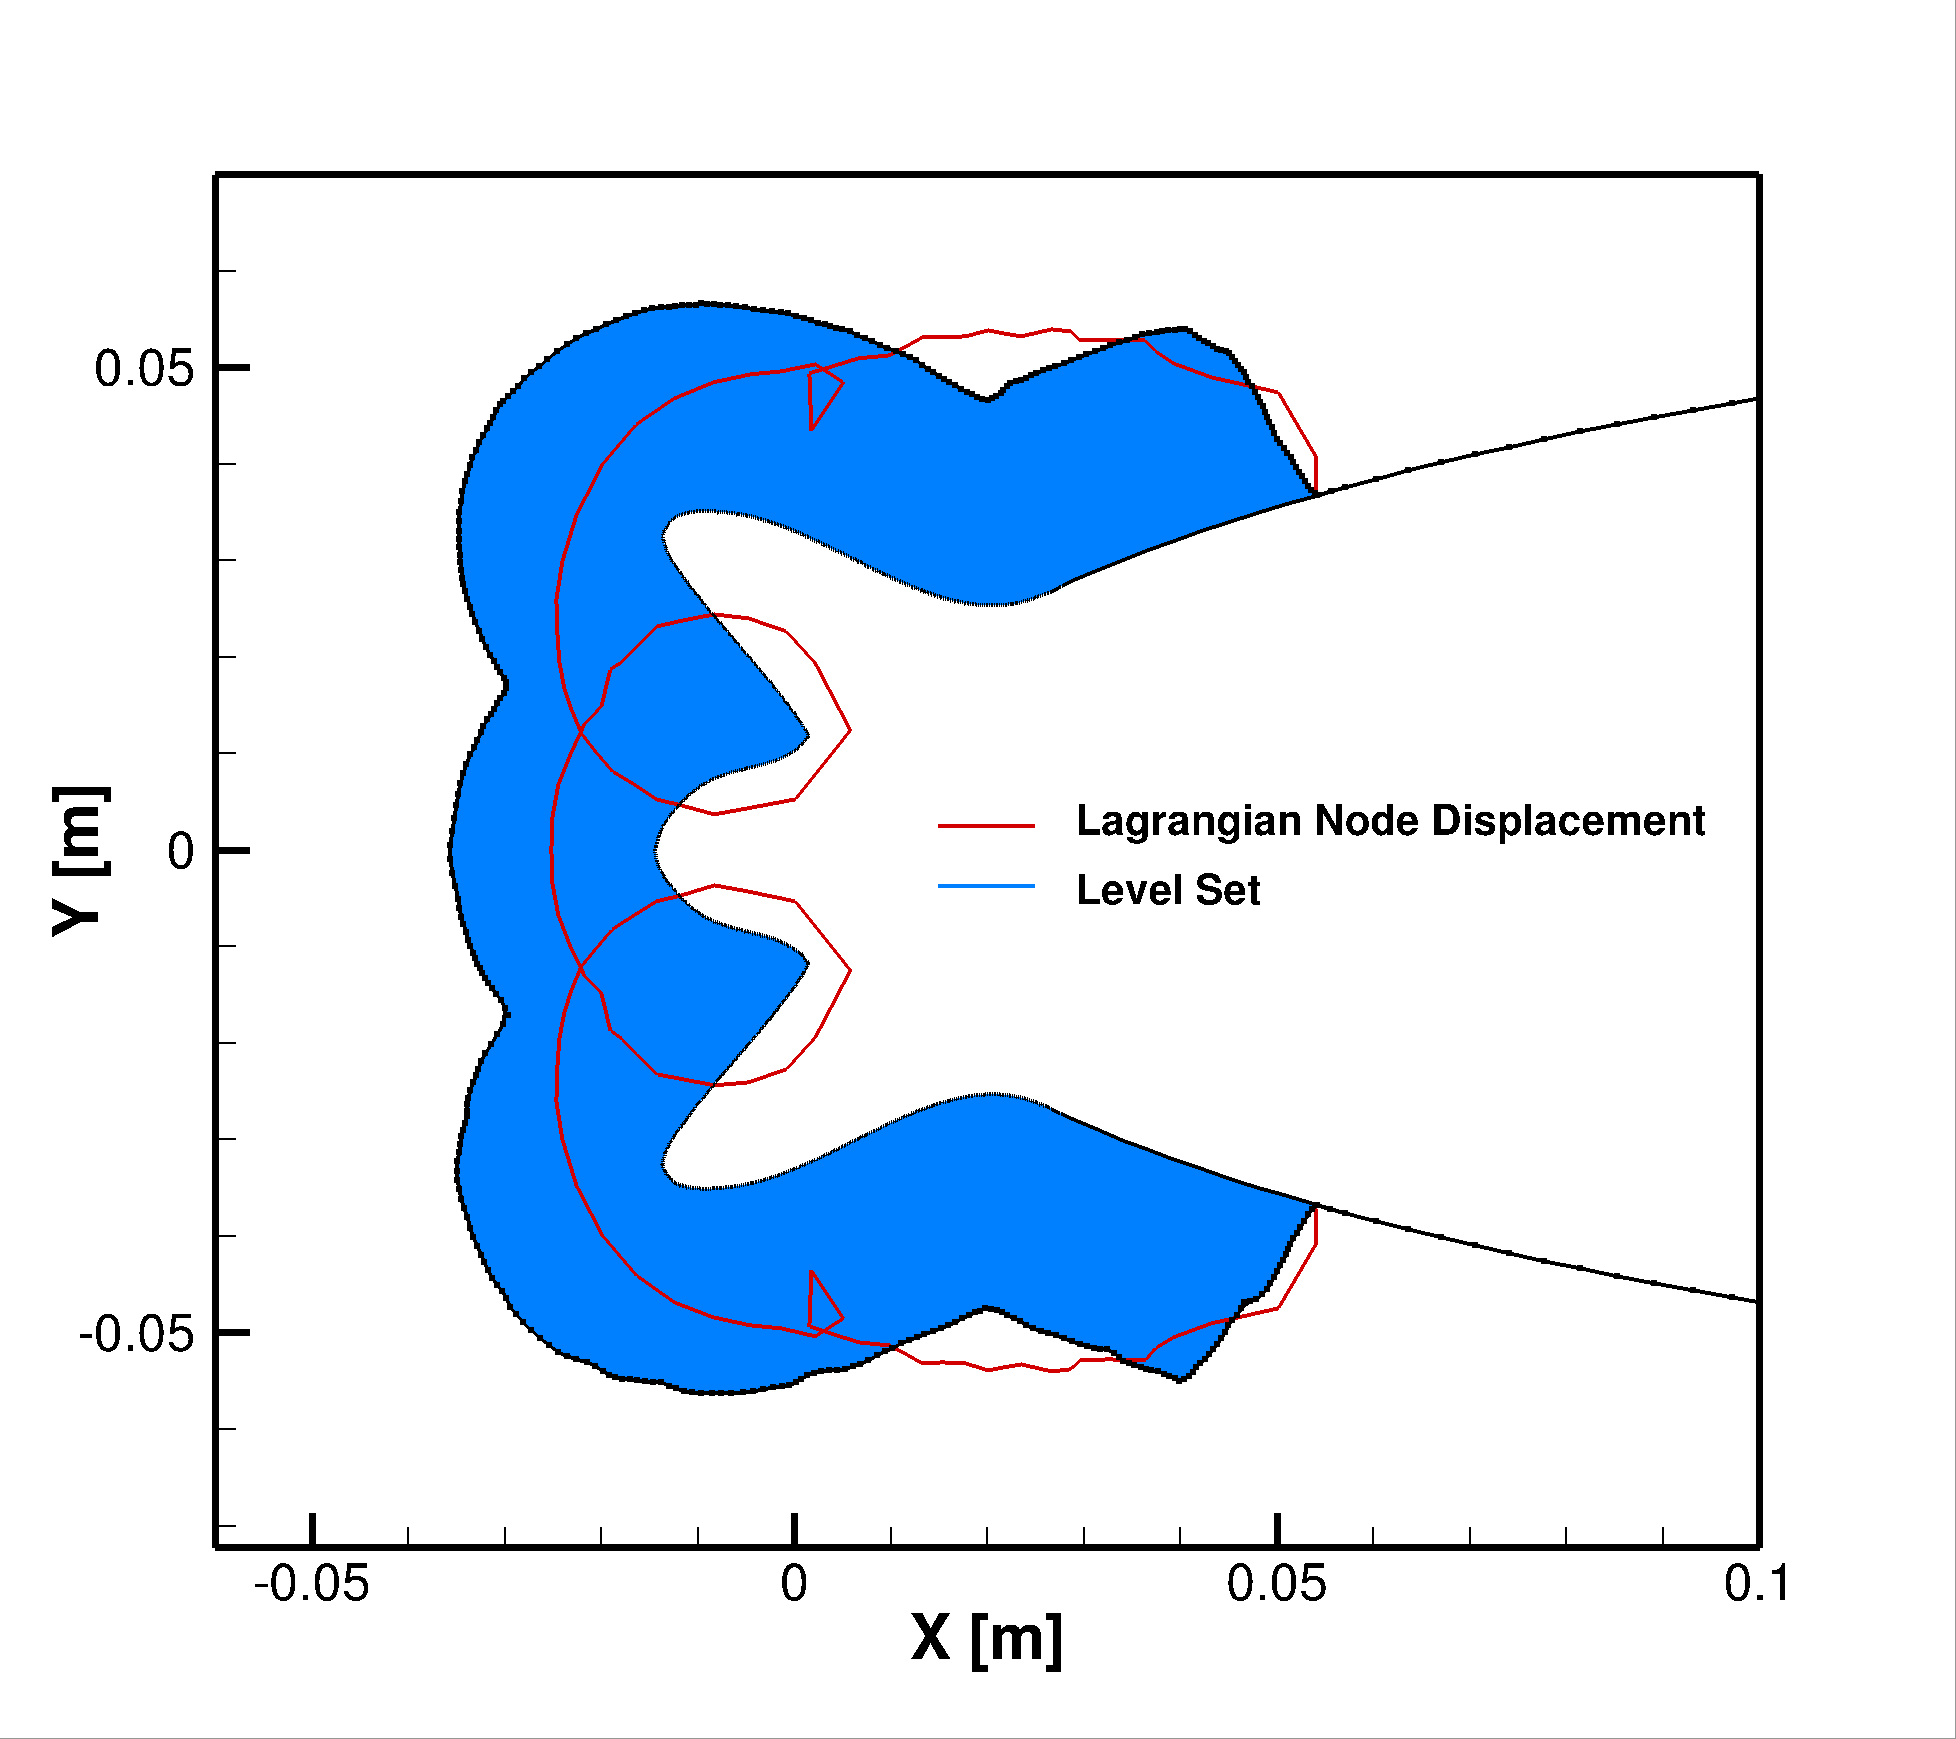
\includegraphics[width=0.68\linewidth]{THREE_HORNS.png}
\caption{Evolution of interacting fronts using surface displacement and the level-set formulation.}
\label{fig:threehorns}
\end{figure}

The methodology is subsequently assessed using two configurations from the AIAA Ice Prediction Workshops \cite{laurendeau2022summary,laurendeau2024summary}. The corresponding icing conditions are summarized in Table~\ref{tab:cases}.

\begin{table}[ht]
\centering
\caption{Summary of the IPW benchmark cases considered in this study.}
\label{tab:cases}
\begin{tabular}{lcc}
\hline
Parameter & Case 241 & Case 362 \\
\hline
Geometry & 2D NACA23012 & 3D swept NACA0012 \\
Icing time (min) & 5.0 & 20.0 \\
LWC (g/m$^3$) & 0.42 & 0.50 \\
MVD ($\mu$m) & 30.0 & 34.7 \\
$M_\infty$ & 0.32 & 0.31 \\
$\alpha$ ($^\circ$) & 2.0 & 0.0 \\
$C_{\mathrm{ref}}$ (in.) & 18 & 36 \\
$T_\infty$ (K) & 250.15 & 266.0 \\
$Re$ & $3.8\times10^6$ & $6.7\times10^6$ \\
\hline
\end{tabular}
\end{table}

% ————————————————————
% IPW1 Case 241
% ————————————————————

\subsection{2D Multilayer Convergence}

IPW1 Case241 corresponds to rime ice accretion on a NACA23012 airfoil and is used to assess the convergence of the multilayer formulation \cite{laurendeau2022summary}. Figure~\ref{fig:case241} compares the predicted ice geometries using 1, 10, and 20 accretion layers with the experimental ice shape.

\begin{figure}[htb]
\centering
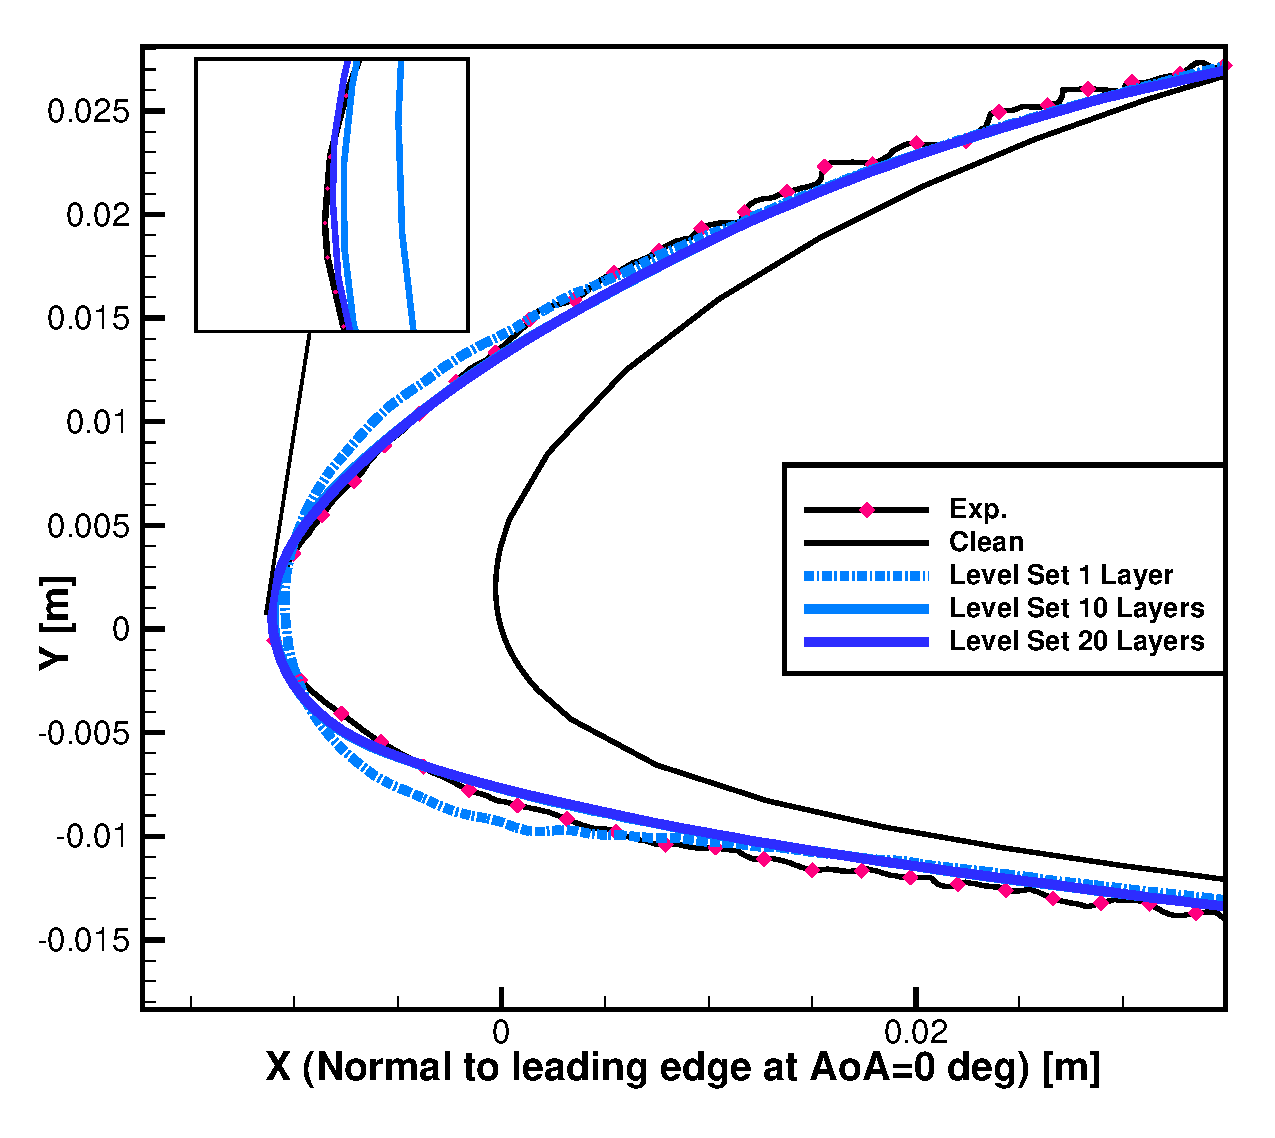
\includegraphics[width=0.82\linewidth]{CASE_IPW1_241_ICE_SHAPE_CONVERGENCE.eps}
\caption{IPW1 Case~241 predictions using 1, 10, and 20 accretion layers.}
\label{fig:case241}
\end{figure}

The experimental maximum ice height is $10.87$~mm. The predicted maximum ice height increases from $10.16$~mm using one layer to $10.69$ and $10.79$~mm using 10 and 20 layers, respectively. The corresponding relative difference with respect to experiment decreases from $6.47\%$ to $1.68\%$ and $0.70\%$. The diminishing difference between the 10- and 20-layer predictions indicates convergence of the predicted ice geometry with increasing temporal resolution.

% ————————————————————
% Case 362
% ————————————————————

\subsection{3D Multilayer Ice Accretion}

The 3D capability of the methodology is assessed using Case362, a swept NACA0012 configuration with a 36-in. chord and a $30^\circ$ sweep angle \cite{diebold2013aerodynamic}. The configuration exhibits spanwise-varying leading-edge ice characteristic of swept-wing icing. The level-set method remains robust throughout the multilayer process, successively advecting, extracting, and remeshing the 3D interface. A 3D view of the predicted ice geometry is shown in Fig.~\ref{fig:case362_3d}.

\begin{figure}[htb]
\centering
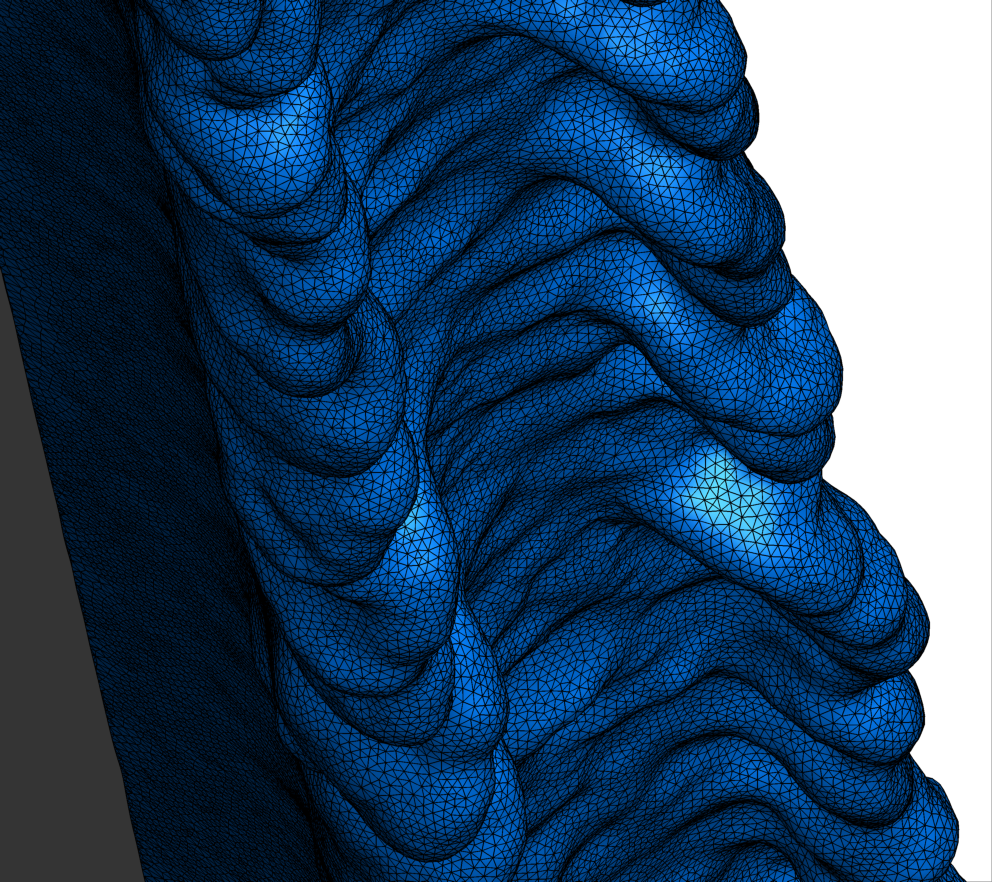
\includegraphics[width=0.82\linewidth]{FIGURES/CLIPPED_ICE_SHAPE_CASE_362_3.png}
\caption{3D view of the predicted ice geometry for Case~362.}
\label{fig:case362_3d}
\end{figure}

The predicted ice geometry shows good agreement with the experimental ice shape and remains within the IPW2 participant envelope \cite{laurendeau2024summary}, as shown in Fig.~\ref{fig:case362_mccs}.

\begin{figure}[htb]
\centering
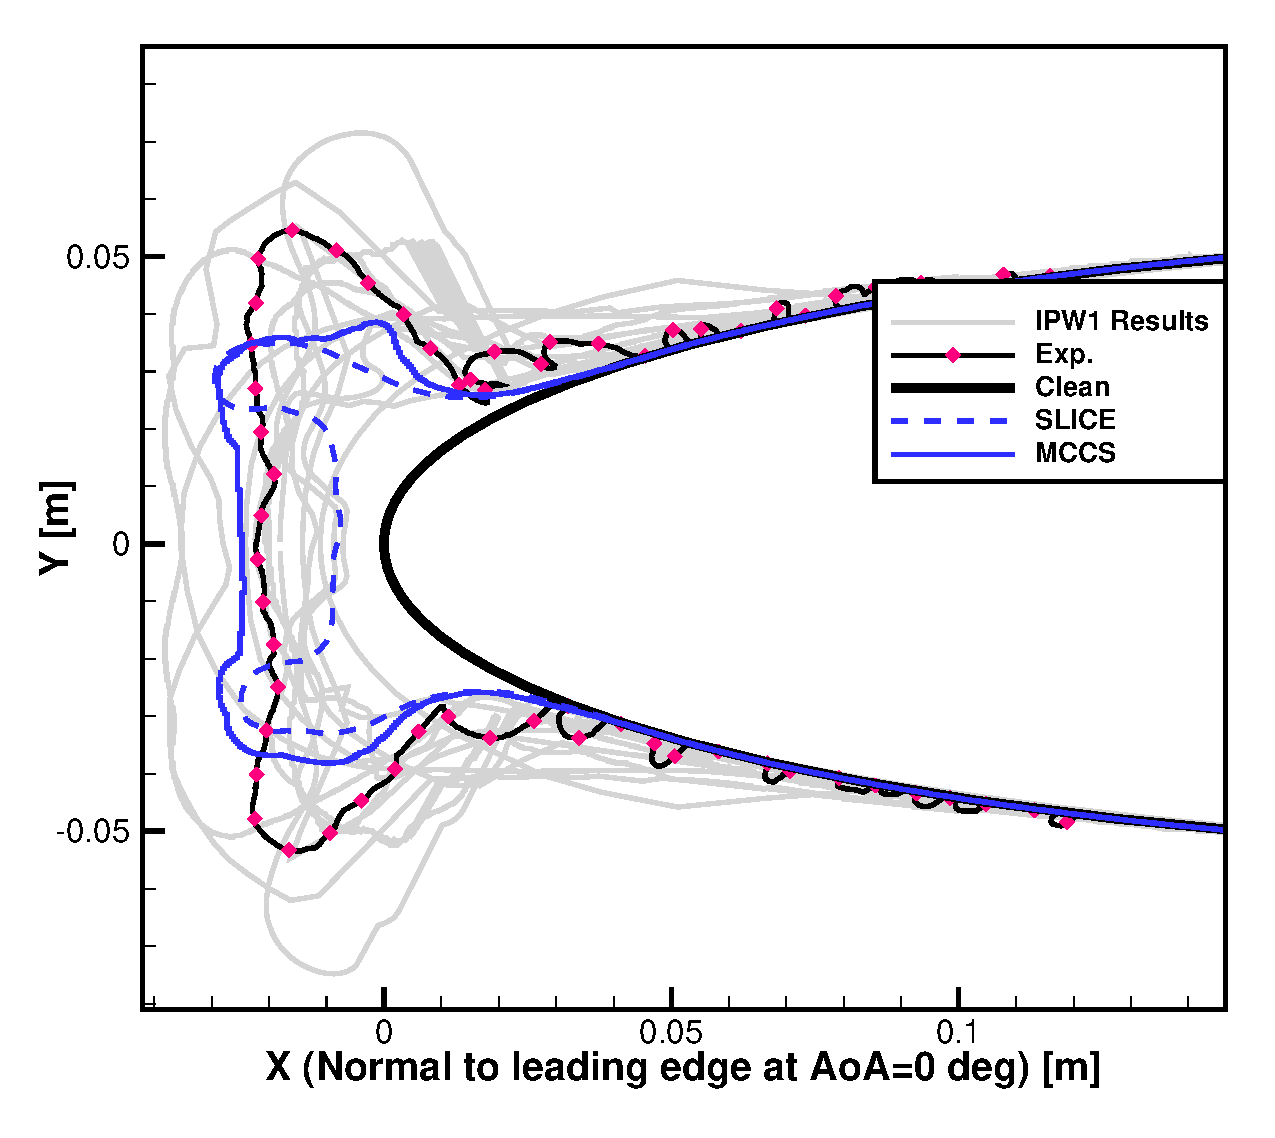
\includegraphics[width=0.82\linewidth]{FIGURES/CASE_IPW1_362_ICE_SHAPE_MCCS_vs_SLICE.eps}
\caption{Comparison of the predicted Case~362 ice geometry with experimental and IPW2 participant data.}
\label{fig:case362_mccs}
\end{figure}


% ============================================================
% EXPECTED RESULTS
% ============================================================

\section{Expected Results}

The completed study will extend the assessment of the level-set methodology to additional configurations from IPW2, with emphasis on complex 3D glaze-ice geometries. These cases will provide further evaluation of the robustness of the interface-propagation, extraction, and remeshing procedure over successive accretion layers. The resulting predictions will be compared with available experimental measurements and workshop participant data to assess ice-shape agreement.


% ============================================================
% CONCLUSION
% ============================================================

% \section{Conclusion}

% A continuous level-set methodology for 2D and 3D multilayer aircraft ice accretion has been developed within \textsc{CHAMPS}. Preliminary results demonstrate that the implicit interface representation can evolve and remesh complex ice geometries without directly displacing the aerodynamic surface. For IPW1 Case~241, increasing the number of layers from 1 to 20 reduces the difference in maximum ice height relative to experiment from $6.47\%$ to $0.70\%$. Application to Case~362 produces 3D ice geometries in good agreement with experiment and within the IPW2 participant envelope while remaining robust throughout the multilayer process. The planned extension to additional IPW2 configurations will further assess the methodology for complex 3D glaze-ice accretion.


\bibliographystyle{ieeetr} % closest to SAE
\bibliography{references}

\section{Contact Information}
Mohamad Karim Zayni, PhD Student\newline
Department of Mechanical Engineering, Polytechnique Montr\'{e}al\newline
mohamad-karim.zayni@polymtl.ca

% ============================================================
% ACKNOWLEDGEMENTS
% ============================================================

\section{Acknowledgements}

This work was supported in part by the Bombardier/NSERC/CRIAQ Industrial Research Chair. Computations were performed on the Trillium supercomputer at the SciNet HPC Consortium, with computational resources provided through the Digital Research Alliance of Canada.


% ============================================================
% DEFINITIONS, ACRONYMS, AND ABBREVIATIONS
% ============================================================

\section{Definitions, Acronyms, Abbreviations}

\begin{table}[h]
\centering
\begin{tabular}{L{0.12\textwidth} L{0.35\textwidth}}
\textbf{GMRES}  & Generalized Minimal Residual \\
\textbf{IPW}    & AIAA Ice Prediction Workshop \\
\textbf{RANS}   & Reynolds-Averaged Navier--Stokes \\
\textbf{ROW}    & Rosenbrock--Wanner \\
\end{tabular}
\end{table}


% ------------------------------------------------------------
% General symbols
% ------------------------------------------------------------

\textbf{General symbols}

\begin{table}[h]
\centering
\begin{tabular}{L{0.10\textwidth} L{0.27\textwidth} L{0.08\textwidth}}
$h_{ice}$                   & Local ice thickness         & $[\mathrm{m}]$ \\
$\boldsymbol{n}_{\phi}$     & Level-set interface normal  & $[-]$ \\
$\Delta t_{\mathrm{layer}}$ & Accretion-layer duration    & $[\mathrm{s}]$ \\
$\boldsymbol{V}_{ice}$      & Ice-growth velocity         & $[\mathrm{m/s}]$ \\
\end{tabular}
\end{table}


% ------------------------------------------------------------
% Greek symbols
% ------------------------------------------------------------

\textbf{Greek symbols}

\begin{table}[h]
\centering
\begin{tabular}{L{0.08\textwidth} L{0.29\textwidth} L{0.08\textwidth}}
$\phi$   & Level-set signed-distance function & $[\mathrm{m}]$ \\
\end{tabular}
\end{table}


\end{document}
